\documentclass[11pt]{article}
\RequirePackage{amssymb, amsfonts, amsmath, latexsym, verbatim, xspace, setspace}
\RequirePackage{tikz, pgflibraryplotmarks}

% By default LaTeX uses large margins.  This doesn't work well on exams; problems
% end up in the "middle" of the page, reducing the amount of space for students
% to work on them.
\usepackage[margin=1in]{geometry}
\usepackage{pgfplots}
\usepackage{hyperref} % FOr URLs
\usepackage[numbers]{natbib} % For citations?  [numbers] needed to avoid Bibliography not compatible with author year citation


\newcommand{\bc}{\mathbf{c}}
\newcommand{\bs}{\mathbf{s}}
\newcommand{\bx}{\mathbf{x}}
\newcommand{\bH}{\mathbf{H}}

\begin{document}
\section{Signal Model}

The signal model is as follows:
\begin{align}
x[t] = A \cos(\omega_0(t-\nu) + \phi) + \epsilon[t] 
\end{align}
for $t = 0, \ldots, T-1$ where $A$ is the signal amplitude, $\omega_0 \in (0,  \pi)$ is the true signal frequency, $\nu = \frac{T-1}{2}$, $\phi$ is the initial signal phase and is uniformly distributed $[0, 2\pi)$, and  $\epsilon$ is an independent, identically normally distributed, zero mean process with variance $\sigma_\epsilon^2$.

The signal-to-noise ratio is given by
\begin{align}
{\tt SNR} =  \frac{A^2}{2 \sigma_\epsilon^2}
\end{align}

\section{Maximum Likelihood Estimation}

Much of this follows Kay's {\bf Example 7.16} in \cite{Kay1997}.

Assuming that the noise $\epsilon$ is normally distributed, then the probability density function of 
\begin{align}
\bx = \Big[x[0], x[1], \ldots, x[T-1] \Big]^T 
\end{align}
is 
\begin{align}
p(\bx ; \mathbf{\theta}) = \frac{1}{(2\pi \sigma_\epsilon^2)^{T/2} }
 \exp\Big(  -\frac{1}{2\sigma_\epsilon^2} \sum_{t=0}^{T-1} \big(x[t] - \tilde{A} \cos(\tilde{\omega}_0(t-\nu) + \tilde{\phi}) \big)^2 \Big)
\end{align}
where our parameters of interest are $\mathbf{\theta} = \Big [ \tilde{A}, \tilde{\omega}_0, \tilde{\phi} \Big ]^T$\footnote{Do we want to add $\sigma_\epsilon^2$?}.

Then we can take the negative logarithm to get
\begin{align}
L(\theta) = \frac{T}{2}\log_e(2\pi \sigma_\epsilon^2)  + \frac{1}{2\sigma_\epsilon^2} \sum_{t=0}^{T-1} \big(x[t] - \tilde{A} \cos(\tilde{\omega}_0(t-\nu) + \tilde{\phi}) \big)^2 
\end{align}
and the maximum likelihood problem because one of {\em minimizing} $L$:
\begin{align}
\hat{\theta} =  \Big [ \hat{A}, \hat{\omega}_0, \hat{\phi} \Big ]^T =  \arg \min_{\theta} L(\theta)
\end{align}

\subsection{Linearizing}

First, Kay~\cite{Kay1997} uses the trigonometric identity
\begin{align}
\cos(A + B) = \cos A \cos B - \sin A \sin B
\end{align}
to rewrite 
\begin{align}
L(\theta)   &= \frac{T}{2}\log_e(2\pi \sigma_\epsilon^2)  + \frac{1}{2\sigma_\epsilon^2} \sum_{t=0}^{T-1} \big(x[t] - \tilde{A} \cos(\tilde{\omega}_0(t-\nu) )\cos(\phi) + \tilde{A} \sin(\tilde{\omega}_0(t-\nu) )\sin(\phi)   \big)^2 \\
L(\theta') &= \frac{T}{2}\log_e(2\pi \sigma_\epsilon^2)  + \frac{1}{2\sigma_\epsilon^2} \sum_{t=0}^{T-1} \big(x[t] - \tilde{\alpha}_c \cos(\tilde{\omega}_0(t-\nu) ) - \tilde{\alpha}_s \sin(\tilde{\omega}_0(t-\nu) )   \big)^2\label{eq:loglikelihoodlinear}
\end{align}
where
\begin{align}
\tilde{\alpha}_c &= \tilde{A} \cos \phi\\
\tilde{\alpha}_s &= -\tilde{A} \sin \phi
\end{align}
So now we've reparamaterized the problem to use
\begin{align}
\theta' = \left [ \tilde{\alpha}_c, \tilde{\alpha}_s, \tilde{\omega}_0\right]^T
\end{align}

\subsection{Vectorizing}

Kay~\cite{Kay1997} takes (\ref{eq:loglikelihoodlinear}) and forms the vector version:
\begin{align}
L(\theta') &=  \frac{T}{2}\log_e(2\pi \sigma_\epsilon^2)  + (\bx  -\tilde{\alpha}_c \bc - \tilde{\alpha}_s \bs )^T  (\bx  -\tilde{\alpha}_c \bc - \tilde{\alpha}_s \bs )\\
&=  \frac{T}{2}\log_e(2\pi \sigma_\epsilon^2)  + (\bx - \bH\underline{\alpha} )^T  (\bx  - \bH \underline{\alpha} )
\end{align}
where
\begin{align}
\bx &= \left [ x[0], x[1], \ldots, x[T-1]  \right]^T\\
\bc &= \left [ \cos\left(-\tilde{\omega}_0 \frac{T-1}{2}\right), \ldots , \cos(-\frac{\tilde{\omega}_0}{2}), \cos(\frac{\tilde{\omega}_0}{2}),   \ldots \cos\left(\tilde{\omega}_0 \frac{T-1}{2}\right) \right]^T\\
\bs &= \left [ \sin\left(-\tilde{\omega}_0 \frac{T-1}{2}\right), \ldots , \sin(-\frac{\tilde{\omega}_0}{2}), \sin(\frac{\tilde{\omega}_0}{2}),   \ldots \sin\left(\tilde{\omega}_0 \frac{T-1}{2}\right) \right]^T\\
\underline{\alpha} &= \left[ \tilde{\alpha}_c\ \tilde{\alpha}_s\right ]^T\\
\bH &= \left [ \bc \ \bs \right ]
\end{align}
assuming $T$ is even.

Kay~\cite{Kay1997}  then notes that this is a least squares problem which, for a given $\bH$ has a solution for $\hat{\underline{\alpha}}$ of
\begin{align}
\hat{\underline{\alpha}} = \left ( \bH^T \bH \right )^{-1} \bH^T \bx
\end{align}

This means
\begin{align}
L(\theta' | \hat{\underline{\alpha}}) &=  \frac{T}{2}\log_e(2\pi \sigma_\epsilon^2)  + (\bx - \bH\hat{\underline{\alpha}} )^T  (\bx  - \bH \hat{\underline{\alpha}} ) \\
&=  \frac{T}{2}\log_e(2\pi \sigma_\epsilon^2)  + (\bx - \bH  \left ( \bH^T \bH \right )^{-1} \bH^T \bx )^T  (\bx  - \bH  \left ( \bH^T \bH \right )^{-1} \bH^T \bx )\\
&= \bx^T \left ( \mathbf{I} -  \bH  \left ( \bH^T \bH \right )^{-1} \bH^T \right) \bx
\end{align}

Which means that the maximum likelihood estimator of frequency can be found by maximizing:
\begin{align}
\bx^T  \bH  \left ( \bH^T \bH \right )^{-1} \bH^T\bx = 
\left [  \begin{matrix} \bc^T \bx \\ \bs^T \bx \end{matrix} \right ]^T
\left [  \begin{matrix} \bc^T \bc  & \bc^T \bs \\ \bs^T \bc & \bs^T \bs \end{matrix} \right ]
\left [  \begin{matrix} \bc^T \bx \\ \bs^T \bx \end{matrix} \right ]\label{eq:mle}
\end{align}

\section{What does this look like?}

Kay~\cite{Kay1997} states near equation (7.66) that when $\omega_0$ is not close to 0 or $\pi$ and when $\bc^T \bc/N \approx \frac{1}{2}$ and $\bs^T \bs/N \approx \frac{1}{2}$ then the MLE of frequency is approximately the same as the periodogram maximizer:
\begin{align}
\hat{\omega}_0 = \arg \max_{\tilde{\omega}_0} \left |  \sum_{t=0}^{T-1} x[t] \exp(-\jmath \tilde{\omega}_0 t) \right |^2\label{eq:per}
\end{align}

So it might be interesting to plot (\ref{eq:mle}) and (\ref{eq:per}) on the same scale.  Figure~\ref{fig:comparison} shows this for the signal
\begin{align}
x[t] = \cos(2\pi 0.0123456789 t + \pi/4) + \cos(2\pi (0.0123456789 + 1/200)t  + \pi/4) + \epsilon[t];
\end{align}
where $T = 32$, and $\epsilon[t]$ is independent and identically normally distributed with zero mean and standard deviation 0.5.

\begin{figure}[h]
\begin{center}
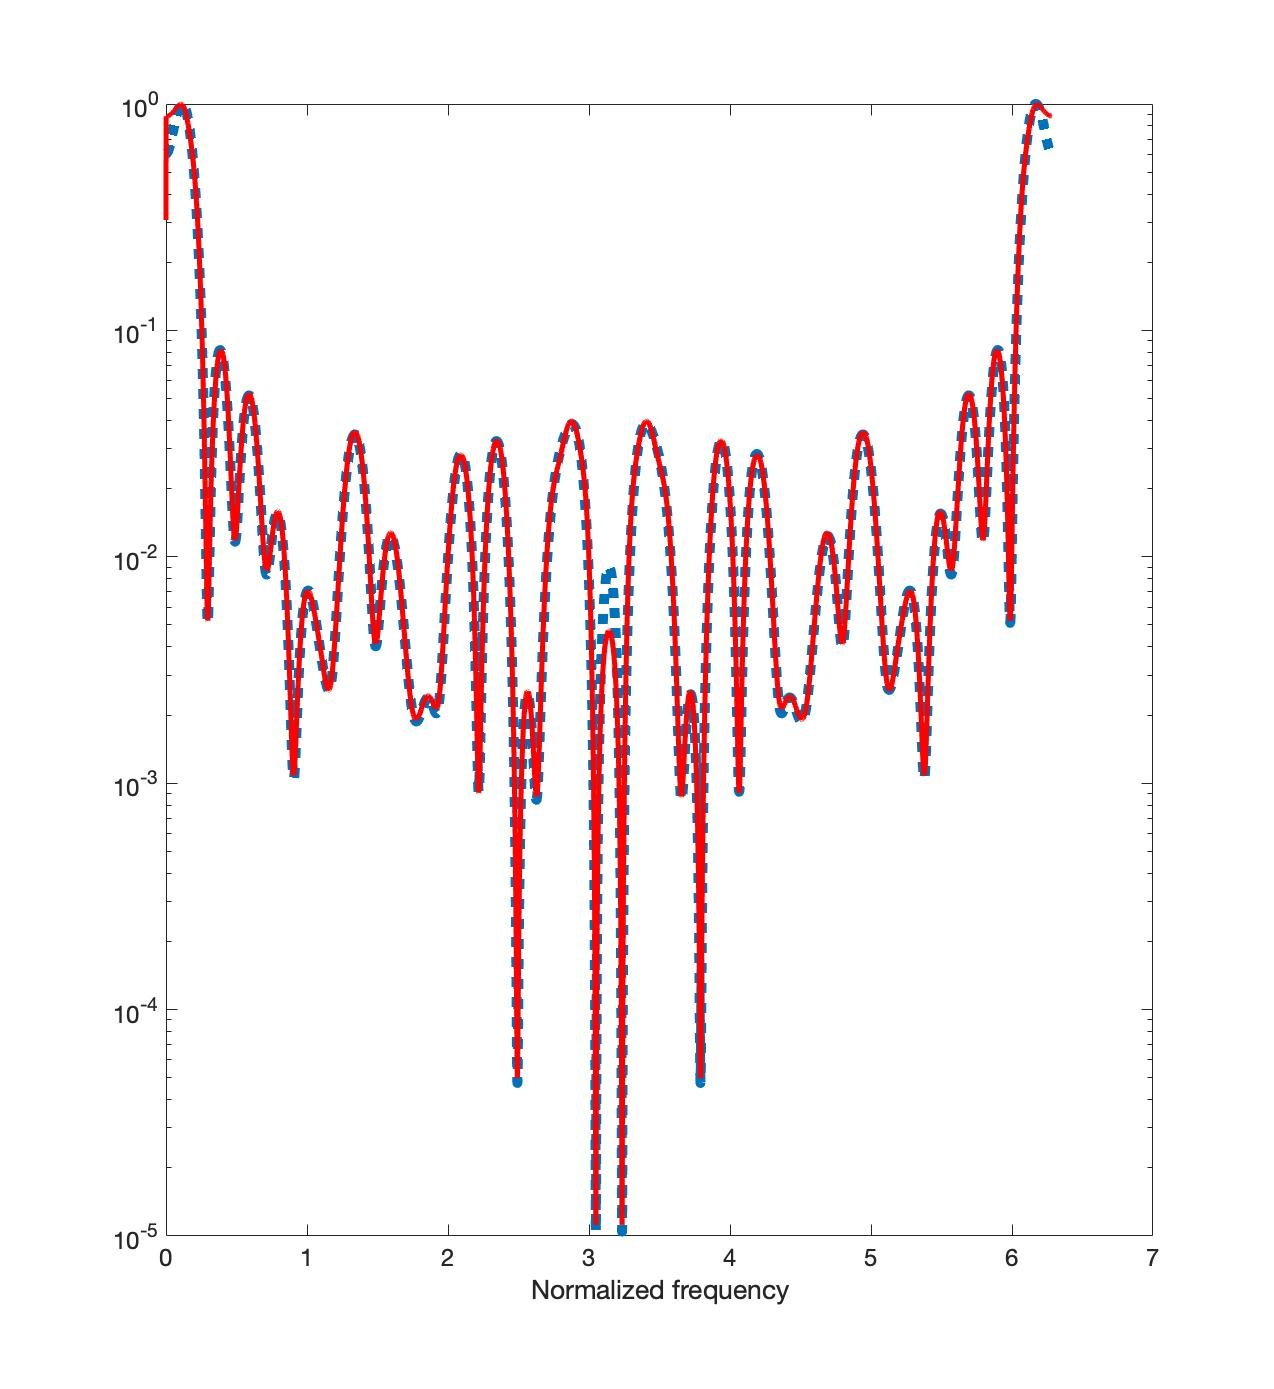
\includegraphics[width=0.3\columnwidth]{comparison-full.jpg}
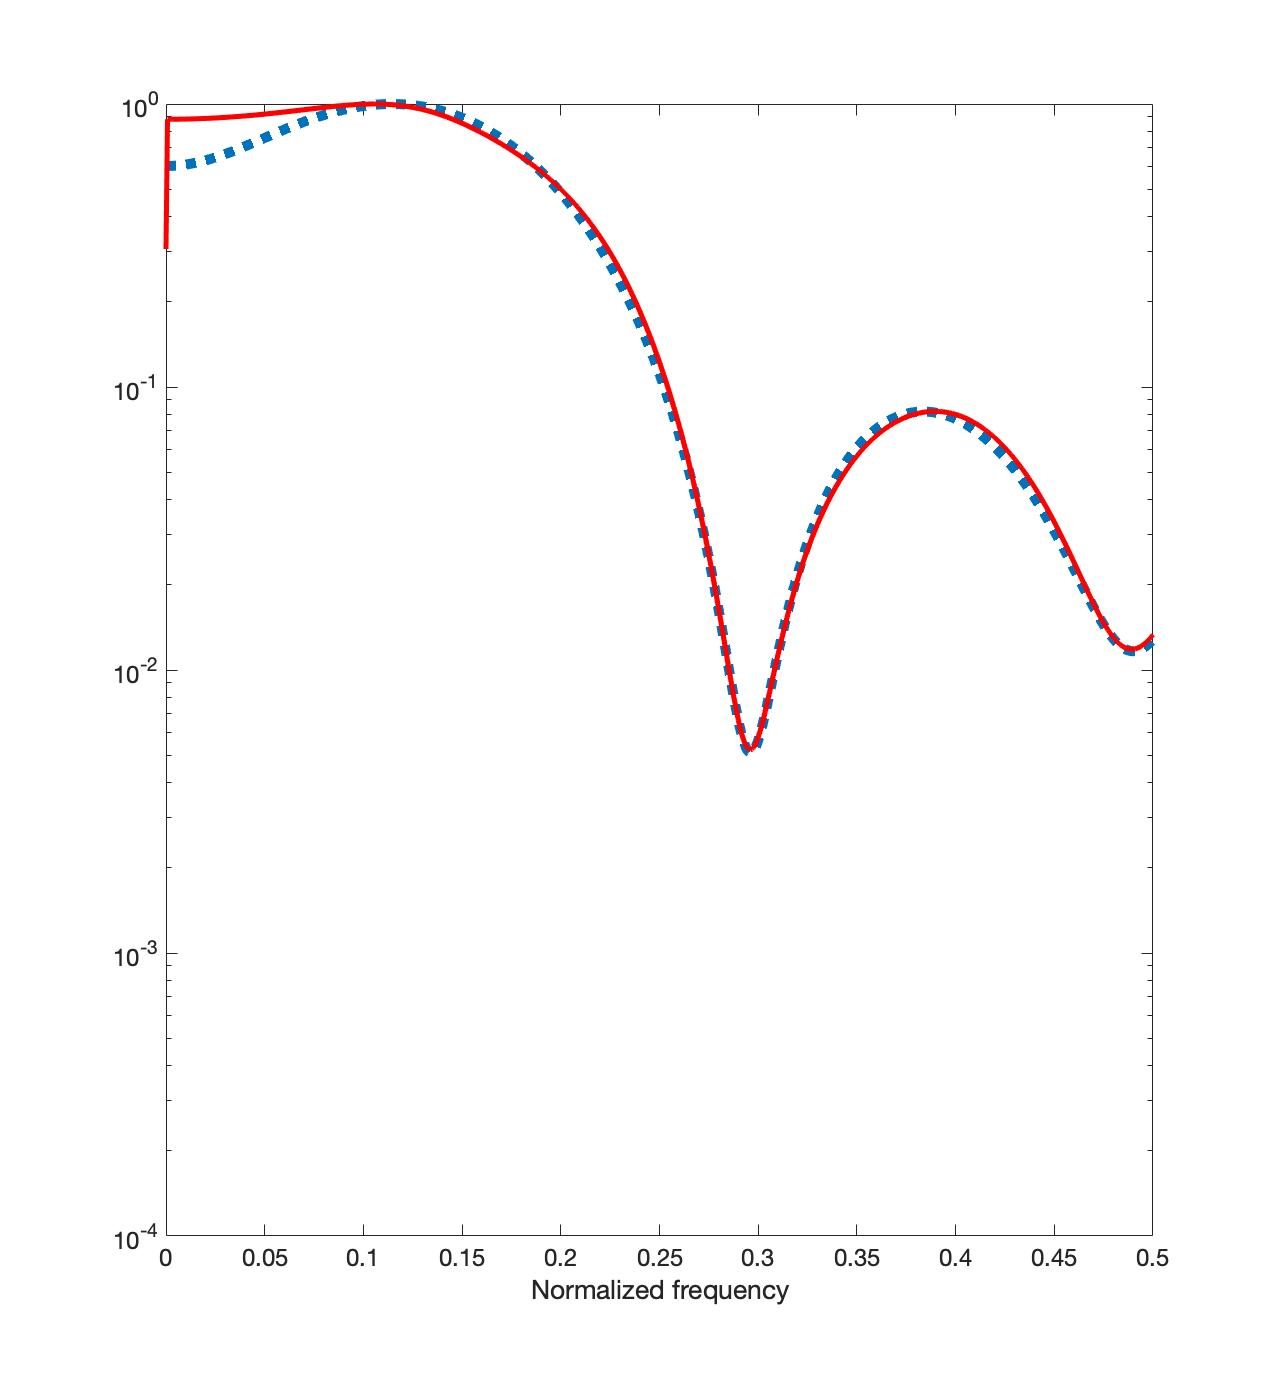
\includegraphics[width=0.3\columnwidth]{comparison-dc.jpg}
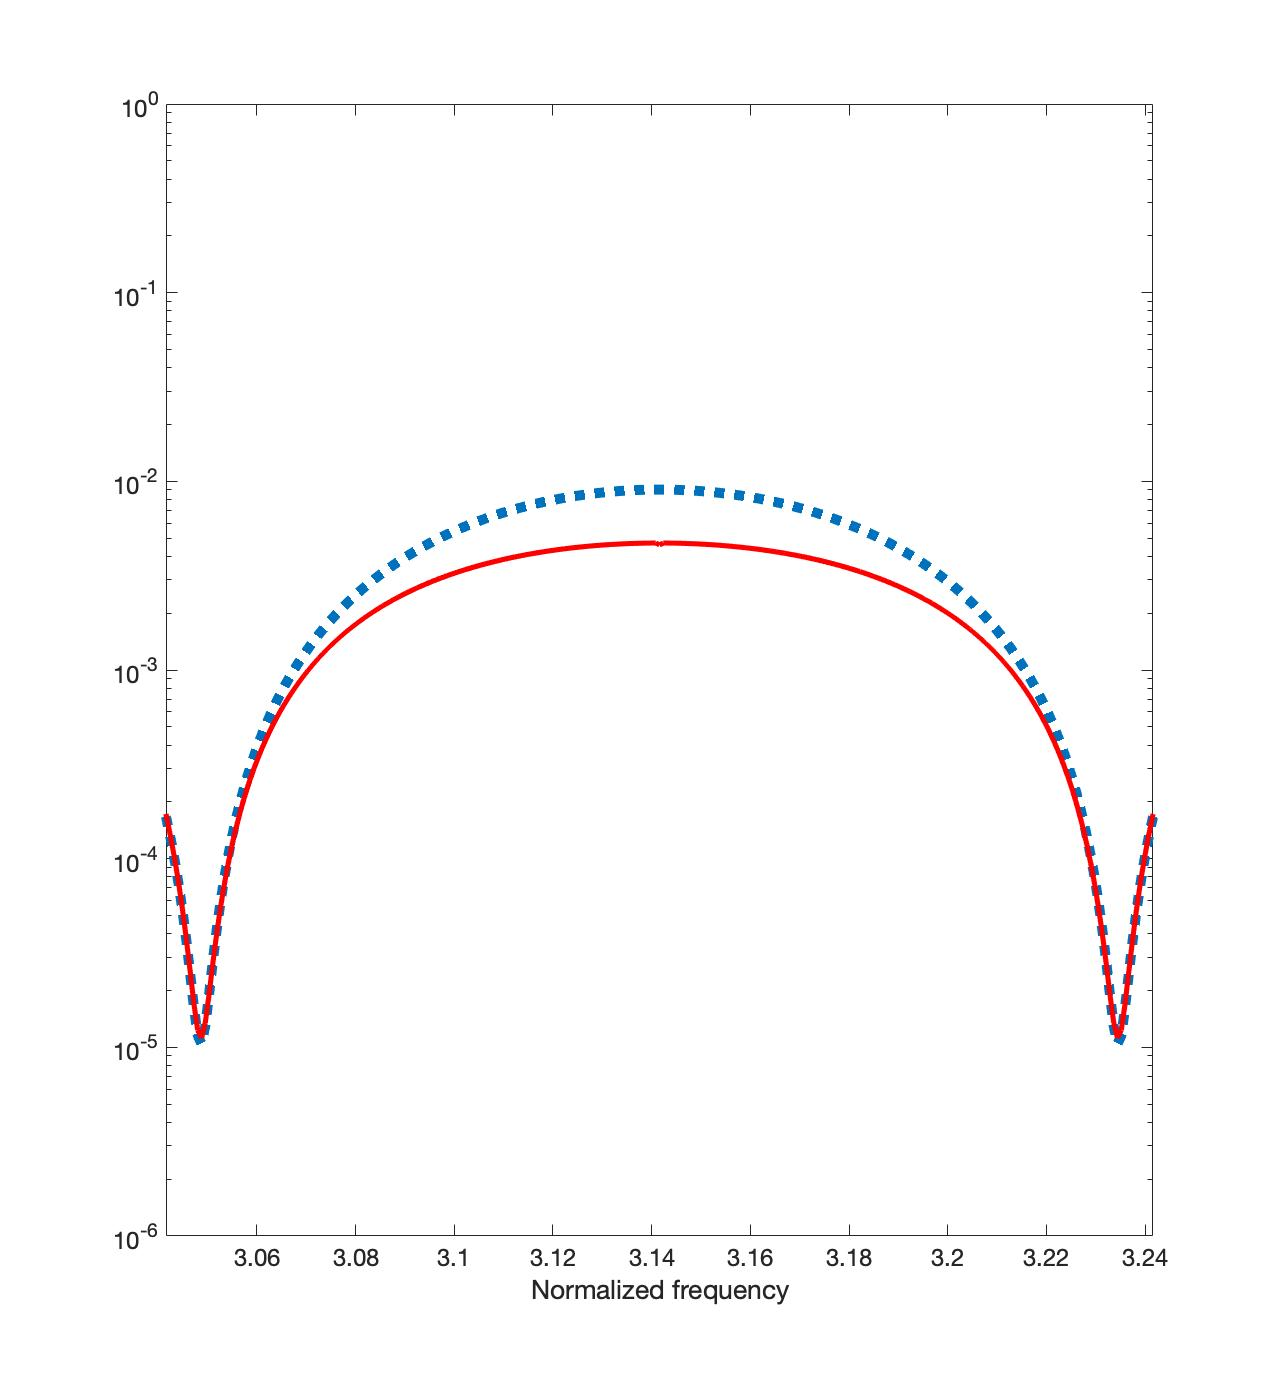
\includegraphics[width=0.3\columnwidth]{comparison-middle.jpg}
\end{center}
\caption{Full frequency range comparison, zoom in around 0, zoom in around $\pi$.}\label{fig:company}\label{fig:comparison}
\end{figure}

\bibliographystyle{ieeetr}
\bibliography{./frequency.bib}


\end{document}

